\documentclass{article}
\usepackage{amsmath}
\usepackage{booktabs}
\usepackage{graphicx}

\begin{document}

\title{Introduction to Spatial Interpolation Techniques}
\author{Frame}
\date{\today}
\maketitle

\section{Inverse Distance Weighting (IDW)}

Inverse Distance Weighting (IDW) is a type of deterministic model for spatial interpolation where the estimated values at a given point are computed as the weighted average of the known values from surrounding points. The weights are inversely related to the distance from the estimation point, emphasizing closer points more significantly.

\subsection{Basic Formula}
The basic formula for IDW is given by:
\[
z(x_0) = \frac{\sum_{i=1}^n \frac{z_i}{d_i^p}}{\sum_{i=1}^n \frac{1}{d_i^p}}
\]
where:
\begin{itemize}
    \item $z(x_0)$ is the interpolated value at location $x_0$.
    \item $z_i$ are the known values at locations $x_i$.
    \item $d_i$ is the distance between $x_0$ and $x_i$.
    \item $p$ is a power parameter that determines the weight; typically, $p = 2$.
\end{itemize}

\subsection{Limitations}
IDW can sometimes produce biased estimates at locations that are far from known data points, or where the spatial distribution of samples is uneven. This leads us to explore more sophisticated methods such as Kriging.

\section{Kriging Method}

Geospatial interpolation the value of a random field at an \emph{unobserved location} from observations other locations. Kriging takes into account both the distance and the \emph{degree of variation between known data points} when estimating values at unknown points.

\subsection{Best Linear Unbiased Prediction (BLUP)}
Incorporates known covariances among observations into the prediction process, ensuring that the predictions are both unbiased (the expected difference between the predicted and true values is zero) and have minimum variance among all linear unbiased predictors. The fundamental assumption in Kriging is that the spatial process underlying the data can be described by a stochastic model, which includes a deterministic mean and a stochastic error process that is spatially correlated.

\subsection{Basic Formulation of Kriging}
The general form of the Kriging estimate is given by a weighted sum of observed values:
\[
Z^*(x_0) = \sum_{i=1}^n \lambda_i Z(x_i)
\]
where:
\begin{itemize}
    \item \(Z^*(x_0)\) is the estimated value at the unobserved location \(x_0\).
    \item \(Z(x_i)\) are the observed values at known locations.
    \item \(\lambda_i\) are the weights assigned to each observed value, which are calculated so as to minimize the variance of the prediction error and ensure the estimator is unbiased.
\end{itemize}

\subsection{Intuitive Pathway to Kriging}

Kriging, unlike simpler methods such as Inverse Distance Weighting, accounts for both the spatial autocorrelation and the variabilities observed in spatial data. Here, we explore a straightforward pathway to understanding how Kriging applies these concepts to improve the accuracy of spatial predictions.

\subsubsection{Understanding Spatial Correlation}
Spatial correlation refers to the statistical relationship between variables located relatively close to each other in space. Kriging utilizes this relationship through the use of a semivariogram, which measures how data similarity decreases as the distance between samples increases.

\textbf{Equation:}
\[
\gamma(h) = \frac{1}{2N(h)} \sum_{i=1}^{N(h)} (Z(x_i) - Z(x_i + h))^2
\]
where \(\gamma(h)\) is the semivariance at lag \(h\), \(Z(x_i)\) is the value at location \(x_i\), and \(N(h)\) is the number of data pairs separated by lag \(h\).

\subsubsection{The Role of Semivariograms}
A semivariogram plots the variance between pairs of sample points as a function of their separation distance. It provides critical insights into the range over which data points influence each other, which directly informs the weighting strategy in Kriging.

\textbf{Practical Example:}
The semivariogram model might look like:
\[
\gamma(h) = C_0 + C(1 - e^{-h/a})
\]
where \(C_0\) is the nugget, \(C\) is the sill, and \(a\) is the range, beyond which points do not influence each other.

\subsubsection{Weights in Kriging}
The essence of Kriging lies in determining optimal weights for the available data points when estimating values at unknown locations. These weights are not merely based on the inverse of the distance (as in IDW) but are derived from solving a system of equations that incorporates the spatial structure as described by the semivariogram. This system ensures that the estimator is unbiased and has the smallest possible variance, making it the Best Linear Unbiased Predictor (BLUP).

\textbf{Equation for Weights:}
\[
\begin{bmatrix}
\gamma(d_{11}) & \gamma(d_{12}) & \dots & \gamma(d_{1n}) & 1 \\
\gamma(d_{21}) & \gamma(d_{22}) & \dots & \gamma(d_{2n}) & 1 \\
\vdots & \vdots & \ddots & \vdots & \vdots \\
\gamma(d_{n1}) & \gamma(d_{n2}) & \dots & \gamma(d_{nn}) & 1 \\
1 & 1 & \dots & 1 & 0
\end{bmatrix}
\begin{bmatrix}
\lambda_1 \\
\lambda_2 \\
\vdots \\
\lambda_n \\
\mu
\end{bmatrix}
=
\begin{bmatrix}
\gamma(d_{10}) \\
\gamma(d_{20}) \\
\vdots \\
\gamma(d_{n0}) \\
1
\end{bmatrix}
\]
where:
\begin{itemize}
    \item $\gamma(d_{ij})$ is the semivariance between points $i$ and $j$.
    \item $d_{ij}$ is the distance between points $i$ and $j$.
    \item $\lambda_i$ are the Kriging weights.
    \item $\mu$ is a Lagrange multiplier used to ensure unbiasedness.
\end{itemize}

\subsubsection{Practical Steps in Kriging}
1. \textbf{Model the semivariogram:} Analyze the collected data to develop a semivariogram that describes how spatial correlation diminishes with distance.
2. \textbf{Solve for Kriging weights:} Use the modeled semivariogram to set up and solve the Kriging equations, which will balance the influence of known data points based on their spatial arrangement and the strength of their interrelationships.
3. \textbf{Estimate values at unsampled locations:} Apply the weights to the known values to estimate unknown values, accounting for both the proximity and the degree of similarity between sampled locations.


\subsection{Radial Basis Function Interpolation}

Radial Basis Function (RBF) interpolation is a widely used method for multivariate interpolation where the value at an unknown point is estimated as a weighted sum of radial basis functions centered at known data points. 

\subsubsection{Formulation}
The interpolated value \( Z^*(x_0) \) at an unobserved location \( x_0 \) is expressed as:
\[
Z^*(x_0) = \sum_{i=1}^n \lambda_i \phi(\|x_0 - x_i\|)
\]
where:
\begin{itemize}
    \item \( \phi \) is the radial basis function, which is a function of the distance between the estimation point and the known data points.
    \item \( \|x_0 - x_i\| \) denotes the Euclidean distance between the unobserved point \( x_0 \) and a known point \( x_i \).
    \item \( \lambda_i \) are the weights calculated through an optimization process that often involves solving a linear system, similarly to how weights are determined in Kriging.
\end{itemize}

\subsubsection{Choice of Radial Basis Function}
Common choices for \( \phi \) include Gaussian, cubic, spline, and multiquadratic radial basis functions. The choice of the function affects the smoothness and fit of the resulting interpolation. Each type of RBF provides different characteristics, and the selection typically depends on the nature of the data and the specific requirements of the analysis.

\subsubsection{Comparison with Kriging}
Unlike Kriging, which explicitly models the spatial correlation and variogram, RBF interpolation focuses more on the form and parameters of the basis function applied. It is an empirical method where the function parameters are often determined by optimization techniques to best fit the spatial distribution of the data.

\subsection{Example Calculations}

\subsubsection{IDW Calculations}
For Inverse Distance Weighting, the interpolated value at the unknown point $(5, 5)$ is calculated using the distances and known values from three points.

\[
\text{Distance Calculation:}
\]
\[
d_i = \sqrt{(x_i - 5)^2 + (y_i - 5)^2}
\]

\[
\text{IDW Weighted Sum:}
\]
\[
z(x_0) = \frac{\sum_{i=1}^3 \frac{z_i}{d_i^2}}{\sum_{i=1}^3 \frac{1}{d_i^2}}
\]

\[
\begin{array}{cccc}
\toprule
x & y & z & \text{Distance from} (5,5) \\
\midrule
1 & 1 & 5 & 5.656854 \\
4 & 3 & 13 & 2.236068 \\
8 & 7 & 6 & 3.605551 \\
\bottomrule
\end{array}
\]

\[
\text{Interpolated value at} (5,5): 10.4415
\]

\subsubsection{Kriging Calculations}
For Kriging, the weights are computed based on the distances and solving the Kriging system. The interpolated value is determined by a linear combination of known values weighted by their spatial relationship to the unknown point.

\[
\begin{array}{ccccc}
\toprule
x & y & z & \text{Distance from} (5,5) & \text{Weights} \\
\midrule
1 & 1 & 5 & 5.656854 & 0.031250 \\
4 & 3 & 13 & 2.236068 & 0.200000 \\
8 & 7 & 6 & 3.605551 & 0.076923 \\
\bottomrule
\end{array}
\]

\[
\text{Interpolated value at} (5,5): 3.2178
\]

\subsection{Visualization}
The interpolation results are visually represented in the following figure. The color scale indicates the value of $z$ at each point, including the interpolated point at $(5, 5)$.

\begin{figure}[H]
\centering
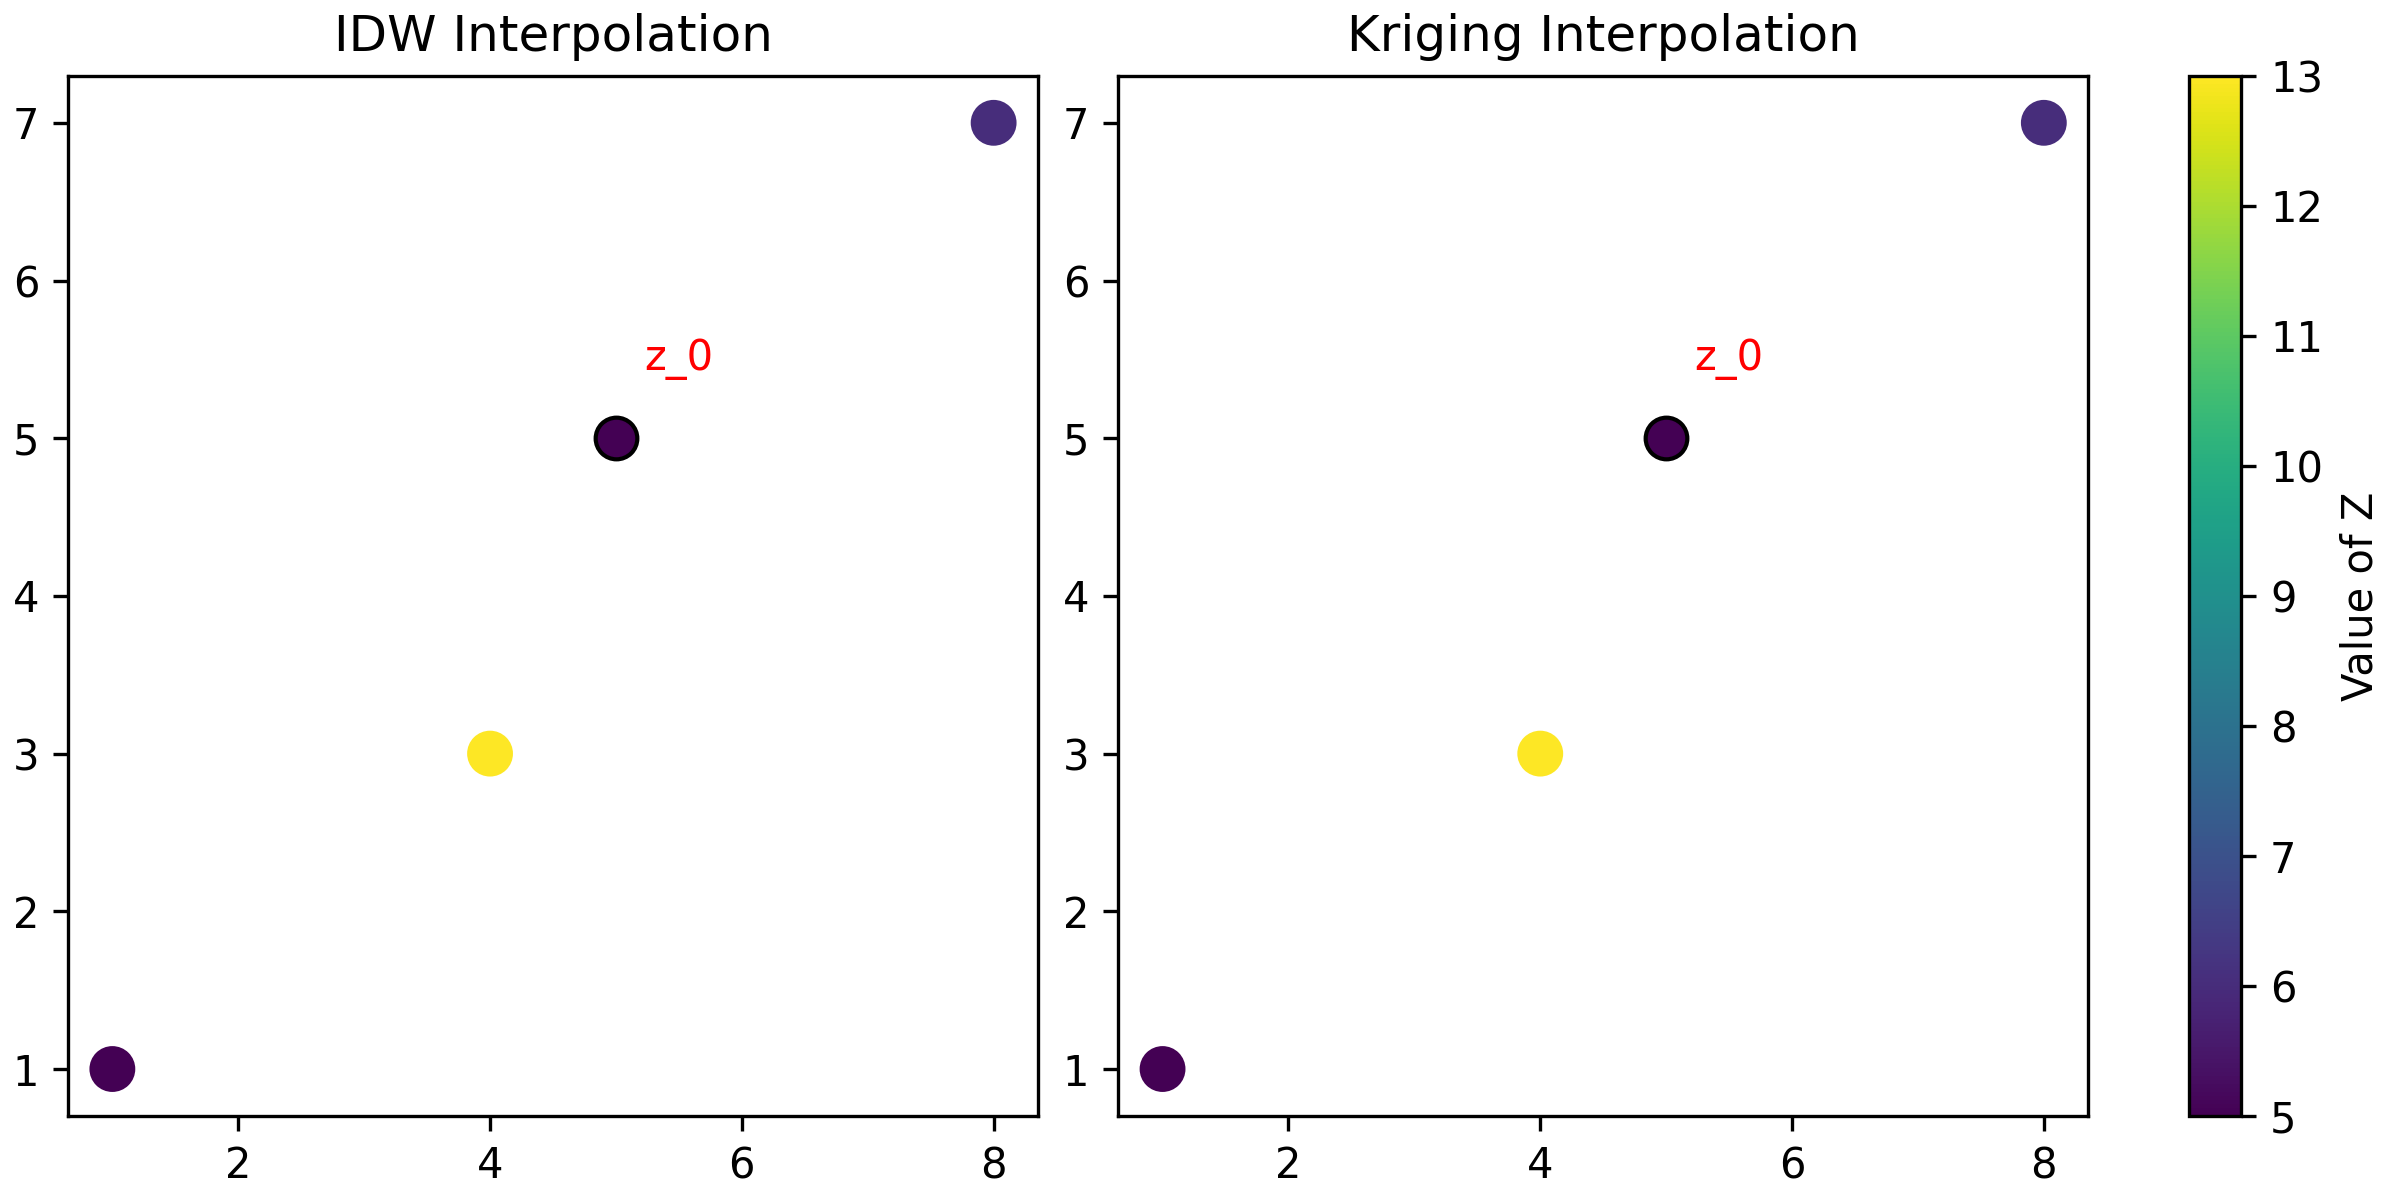
\includegraphics[width=0.8\textwidth]{spatial_interpolation.png}
\caption{IDW and Kriging interpolation visualizations.}
\end{figure}


\end{document}